%%%%%%%%%%%%%%%%%%%%%%%%%%%%%%%%%%%%%%%%%%%%%%%%%%%%%%%%%%%%%%%%%%%%%%%%
%%% AAMAS-2024 paper -- Conformal Replay for Off-Policy MARL
%%% Built on the official AAMAS-2024 sigconf template.
%%% Switch to the anonymous variant below for double-blind submission.
%%%%%%%%%%%%%%%%%%%%%%%%%%%%%%%%%%%%%%%%%%%%%%%%%%%%%%%%%%%%%%%%%%%%%%%%

\documentclass[sigconf]{aamas}
%\documentclass[sigconf,anonymous]{aamas} % <- use this one for submission

\usepackage{balance}      % for balancing columns on the final page
\usepackage{amsmath}
\usepackage{mathtools}   % loads amsmath; amssymb is already provided by the ACM newtx fonts (avoids the \Bbbk clash)
\usepackage{bm}
\usepackage{algorithm}
\usepackage{algpseudocode}

\graphicspath{{imgs/}{imgs/results/}{imgs/new_results/}{imgs/logo/}}

%%% AAMAS-2024 copyright block (do not change!)
\setcopyright{ifaamas}
\acmConference[AAMAS '24]{Proc.\@ of the 23rd International Conference
on Autonomous Agents and Multiagent Systems (AAMAS 2024)}{May 6 -- 10, 2024}
{Auckland, New Zealand}{N.~Alechina, V.~Dignum, M.~Dastani, J.S.~Sichman (eds.)}
\copyrightyear{2024}
\acmYear{2024}
\acmDOI{}
\acmPrice{}
\acmISBN{}
\acmSubmissionID{<<EasyChair submission id>>}

%%%%%%%%%%%%%%%%%%%%%%%%%%%%%%%%%%%%%%%%%%%%%%%%%%%%%%%%%%%%%%%%%%%%%%%%
%%% Author-defined commands
\newcommand{\BibTeX}{\rm B\kern-.05em{\sc i\kern-.025em b}\kern-.08em\TeX}

\newcommand{\uma}{\mathbf{u}_{-a}}
\newcommand{\umai}{\mathbf{u}_{i,-a}}
\newcommand{\picur}{\pi^{\mathrm{cur}}_{-a}}
\newcommand{\pipast}{\pi^{\mathrm{past}}_{-a}}
\newcommand{\pipasti}{\pi^{\mathrm{past}}_{i,-a}}
\newcommand{\Qbr}{Q^{\mathrm{BR}}_{a}}
\newcommand{\Dcal}{\mathcal{D}}
\newcommand{\Ccal}{\mathcal{C}}
\newcommand{\Bop}{\mathcal{B}}
\newcommand{\indic}[1]{\mathbf{1}\!\left[#1\right]}
\DeclareMathOperator*{\argmax}{arg\,max}
\DeclareMathOperator{\supp}{supp}

%%%%%%%%%%%%%%%%%%%%%%%%%%%%%%%%%%%%%%%%%%%%%%%%%%%%%%%%%%%%%%%%%%%%%%%%

\title{Conformal Replay for Off-Policy Multi-Agent Reinforcement Learning}

\author{Arnaud Gardille}
\affiliation{%
  \institution{ENS Paris-Saclay}
  \city{Gif-sur-Yvette}
  \country{France}}
\email{arnaud.gardille@gmail.com}

\author{Thibault Lahire}
\affiliation{%
  \institution{Dassault Aviation}
  \city{Saint-Cloud}
  \country{France}}
\email{thibault.lahire@dassault-aviation.com}

\begin{abstract}
In off-policy multi-agent reinforcement learning (MARL), each agent perceives
the other learners as part of its environment; as their policies drift, the
perceived dynamics become non-stationary and previously collected transitions
turn misleading. The usual remedy---shrinking the replay buffer---discards the
sample efficiency that motivates off-policy learning in the first place. We
recast the \emph{staleness} of a stored transition as a question of
\emph{conformity} to the other agents' \emph{current} policies, and answer it
with conformal prediction. We define a non-conformity score that measures how
surprising a transition is under the agents' current policies---or, when those
policies are unavailable, under a model of the currently perceived
dynamics---calibrate it on fresh transitions, and obtain distribution-free
$p$-values. These $p$-values serve two purposes: (i)~a large-batch-then-subsample
\emph{selection} rule that biases learning towards transitions compatible with
the present, generalising importance-ratio prioritisation to settings where the
ratio is unavailable or numerically unstable; and (ii)~a conformal
\emph{test martingale} that detects, with an anytime false-alarm guarantee via
Ville's inequality, when the perceived environment has drifted enough to
invalidate the buffer. We formalise the perceived best-response value that these
schemes target, clarify the (self-normalised, deliberately biased) nature of
ratio prioritisation, and study the approach on two controlled cooperative
environments designed to isolate perceived non-stationarity.
\end{abstract}

\ccsdesc[500]{Computing methodologies~Multi-agent reinforcement learning}
\ccsdesc[500]{Computing methodologies~Sequential decision making}
\ccsdesc[300]{Mathematics of computing~Hypothesis testing and confidence interval computation}

\keywords{Multi-agent reinforcement learning; Off-policy learning; Experience
replay; Non-stationarity; Conformal prediction; Sequential change detection}

%%%%%%%%%%%%%%%%%%%%%%%%%%%%%%%%%%%%%%%%%%%%%%%%%%%%%%%%%%%%%%%%%%%%%%%%

\begin{document}

\pagestyle{fancy}
\fancyhead{}

\maketitle

%%%%%%%%%%%%%%%%%%%%%%%%%%%%%%%%%%%%%%%%%%%%%%%%%%%%%%%%%%%%%%%%%%%%%%%%
\section{Introduction}

Many domains---robotics, logistics, healthcare, finance, and strategy
games---could benefit from agents that learn to act together. Yet, in spite of
impressive results on benchmarks such as the StarCraft Multi-Agent
Challenge~\cite{samvelyan2019starcraft}, multi-agent reinforcement learning
(MARL) remains hard to deploy because of slow and unstable
convergence~\cite{matignon2012independent}.

A large part of this difficulty has a single, well-identified cause. Single-agent
reinforcement learning assumes a \emph{stationary} environment. In MARL, from the
point of view of one agent, the other agents are part of the environment; as they
update their policies, the dynamics that the agent perceives \emph{change over
time}. This \emph{perceived non-stationarity}~\cite{matignon2012independent} is
particularly damaging for \emph{off-policy}, value-based methods, which owe their
sample efficiency to a \emph{replay buffer}: they repeatedly learn from
transitions collected long ago, under \emph{outdated} policies of the other
agents. A common workaround is to keep the buffer small, so that stale
transitions are quickly forgotten---but this throws away exactly the sample
efficiency and the offline-learning capability that motivate off-policy learning.

The key observation of this paper is that \emph{old does not imply useless}. A
stored transition is harmful only insofar as the joint action taken by the other
agents in it is \emph{implausible under their current policies}. If their stored
behaviour is still compatible with what they would do now, the transition is as
informative as a fresh one. The problem of reusing the past therefore reduces to
a problem of \emph{selecting transitions that conform to the present}.

Prior work makes this concrete through an importance-sampling ratio between the
current and past probabilities of the other agents'
actions~\cite{foerster2017stabilising}. We revisit that idea, fix its
mathematical formulation, and show that the ratio is often either
\emph{unavailable} (partial observability, continuous actions, parametric
exploration, black-box teammates) or \emph{numerically unstable} (its variance
explodes). We then replace the explicit ratio by a \emph{calibrated,
distribution-free measure of conformity} drawn from conformal
prediction~\cite{vovk2005algorithmic,angelopoulos2023gentle}.

\paragraph{Contributions.}
\begin{enumerate}
  \item We formalise the value that off-policy MARL implicitly targets as a
  \emph{best-response value} against the other agents' current policies, and make
  explicit the quasi-stationary approximation it relies on
  (Section~\ref{sec:formulation}, Appendix~\ref{app:br}).
  \item We give a corrected account of importance-ratio reweighting: the
  change-of-measure identity and its support condition, the heavy-tailed
  instability of direct loss correction, and the fact that ratio
  \emph{prioritisation} is a \emph{self-normalised}, deliberately biased estimator
  rather than an unbiased one (Section~\ref{sec:formulation}).
  \item We introduce \emph{conformal replay}: a non-conformity score for stored
  transitions, calibrated into $p$-values, used both to \emph{select} compatible
  transitions (Section~\ref{sec:selection}) and to \emph{detect} drift of the
  perceived environment through a conformal test martingale with an anytime
  false-alarm guarantee (Section~\ref{sec:detection}).
  \item We describe two controlled cooperative environments that isolate
  perceived non-stationarity, and report the motivating evidence together with an
  evaluation protocol (Section~\ref{sec:experiments}, Appendix~\ref{app:reward}).
\end{enumerate}

%%%%%%%%%%%%%%%%%%%%%%%%%%%%%%%%%%%%%%%%%%%%%%%%%%%%%%%%%%%%%%%%%%%%%%%%
\section{Background and Notation}
\label{sec:background}

\subsection{Reinforcement learning}
A Markov Decision Process (MDP) is a tuple $(S,A,P,R,\gamma)$ with state set $S$,
action set $A$, transition kernel $P(\cdot\mid s,a)\in\Delta(S)$, reward
distribution $R(\cdot\mid s,a)$, and discount $\gamma\in[0,1)$. A policy
$\pi:S\to\Delta(A)$ induces a return $\sum_{t\ge0}\gamma^t R_{t}$, and the
action-value function $Q_\pi(s,a)=\mathbb{E}_\pi[\sum_{t\ge0}\gamma^tR_t\mid
S_0=s,A_0=a]$. The optimal value $Q^*=\max_\pi Q_\pi$ is the unique fixed point
of the optimal Bellman operator
\begin{equation}
\label{eq:bellman}
(\Bop^* Q)(s,a)=\mathbb{E}_{s'\sim P(\cdot\mid s,a)}\Big[R(s,a,s')+\gamma
\max_{a'}Q(s',a')\Big],
\end{equation}
which is a $\gamma$-contraction for $\lVert\cdot\rVert_\infty$
(Appendix~\ref{app:contraction}). Note that the right-hand side uses $Q$, not
$Q^*$: $\Bop^*$ maps an arbitrary $Q$ to a new function, and iterating it
converges to $Q^*$ by Banach's theorem.

\paragraph{Deep $Q$-learning.}
DQN~\cite{mnih2013playing} parameterises $Q_\phi$ by a neural network, stores
transitions in a replay buffer $\Dcal$, and minimises, over uniformly sampled
batches,
\begin{equation}
\label{eq:dqn}
\mathcal{L}(\phi)=\mathbb{E}_{(s,a,r,s')\sim U(\Dcal)}\Big[\big(Q_\phi(s,a)-y\big)^2\Big],
\quad y=r+\gamma\max_{a'}Q_{\bar\phi}(s',a'),
\end{equation}
with $\bar\phi$ a periodically updated target network. A stochastic gradient step
on a batch of size $B$ reads
\begin{equation}
\label{eq:sgd}
\phi\;\leftarrow\;\phi-\alpha\,\nabla_\phi\frac1B\sum_{i=1}^{B}\big(y_i-Q_\phi(s_i,a_i)\big)^2 .
\end{equation}
Exploration typically uses an $\epsilon$-greedy policy: act greedily w.p.\
$1-\epsilon$ and uniformly at random w.p.\ $\epsilon$.

\subsection{Multi-agent reinforcement learning}
A cooperative \emph{stochastic game} is a tuple
$(N,S,(\mathbb{U}_a)_{a=1}^N,\mathcal{T},(r_a)_{a=1}^N,\gamma)$: $N$ agents share
the state $s\in S$, agent $a$ picks $u_a\in\mathbb{U}_a$, the joint action
$\mathbf{u}=(u_a,\uma)$ drives the transition
$\mathcal{T}(\cdot\mid s,\mathbf{u})$ and the reward $r_a(s,\mathbf{u})$. We
write $a$ for the agent under consideration and $-a$ for the others, so that
$u_a\sim\pi_a(\cdot\mid s)$ and $\uma\sim\pi_{-a}(\cdot\mid s)$.

\paragraph{Independent $Q$-learning (IQL).}
In IQL~\cite{tampuu2017multiagent} each agent runs its own DQN, treating the
others as part of the environment. Its loss is
\begin{equation}
\label{eq:iql}
\mathcal{L}_a(\phi_a)=\mathbb{E}_{(s,\mathbf{u},r,s')\sim U(\Dcal)}
\Big[\big(Q_{\phi_a}(s,u_a)-y_a\big)^2\Big],
\end{equation}
\[
y_a=r_a+\gamma\max_{u_a'}Q_{\bar\phi_a}(s',u_a').
\]
IQL is simple and, despite its non-stationarity, underlies competitive
value-decomposition methods such as VDN~\cite{sunehag2018value} and
QMIX~\cite{rashid2018qmix}; the mechanisms we develop apply to those methods
unchanged, since each agent still maintains an individual $Q$-function. We adopt
the fully observable, simultaneous-action setting for clarity; the partially
observable case is discussed in Section~\ref{sec:conclusion}.

%%%%%%%%%%%%%%%%%%%%%%%%%%%%%%%%%%%%%%%%%%%%%%%%%%%%%%%%%%%%%%%%%%%%%%%%
\section{The Replay Mismatch in MARL}
\label{sec:formulation}

\subsection{The perceived MDP and the best-response value}
Fix agent $a$ and freeze the others at a joint policy $\pi_{-a}$. From $a$'s
viewpoint the game collapses to an MDP $\mathcal{M}_a(\pi_{-a})$ with
\emph{perceived} transition and reward kernels
\begin{align}
P^{\pi_{-a}}(s'\mid s,u_a)&=\mathbb{E}_{\uma\sim\pi_{-a}(\cdot\mid s)}\big[\mathcal{T}(s'\mid s,u_a,\uma)\big],\\
\bar r^{\pi_{-a}}(s,u_a)&=\mathbb{E}_{\uma\sim\pi_{-a}(\cdot\mid s)}\big[r_a(s,u_a,\uma)\big].
\end{align}
The value that IQL implicitly chases is the optimal value of this perceived MDP,
i.e.\ the \emph{best response} of agent $a$ to $\pi_{-a}$, defined as the fixed
point of the best-response Bellman operator
\begin{equation}
\label{eq:br}
(\Bop^{\mathrm{BR}}_{\pi_{-a}}Q)(s,u_a)=
\mathbb{E}_{\uma\sim\pi_{-a}(\cdot\mid s),\,s'\sim\mathcal{T}}
\Big[r_a(s,\mathbf{u})+\gamma\max_{u_a'}Q(s',u_a')\Big].
\end{equation}
We denote its fixed point $\Qbr(s,u_a;\pi_{-a})$. For \emph{fixed} $\pi_{-a}$,
$\Bop^{\mathrm{BR}}_{\pi_{-a}}$ is a $\gamma$-contraction
(Appendix~\ref{app:br}), so $\Qbr(\cdot;\pi_{-a})$ is well defined.

This is a \emph{best-response} value, \emph{not} a joint-optimal or equilibrium
value: it is optimal for $a$ \emph{only against the fixed} $\pi_{-a}$. During
training the others keep learning, so the relevant target is
$\Qbr(\cdot;\picur)$ with $\picur$ \emph{moving}. Off-policy MARL thus rests on a
\emph{quasi-stationary} approximation: at each update we treat the current others'
policies as fixed. Perceived non-stationarity is precisely the drift of this
target, and it is what makes a fixed buffer inconsistent.

\subsection{What exactly is mismatched}
The buffer stores transitions $\tau_i=(s_i,u_{i,a},\umai,r_i,s_i')$ in which the
others' actions were drawn from their \emph{past} policy,
$\umai\sim\pipasti(\cdot\mid s_i)$. The loss we would \emph{like} to minimise
draws them from the \emph{current} policy:
\begin{align}
\label{eq:loss-ideal}
\mathcal{L}^{\mathrm{cur}}_a(\phi_a)&=
\mathbb{E}_{\,\uma\sim\picur(\cdot\mid s)}\Big[\big(Q_{\phi_a}(s,u_a)-y_a\big)^2\Big],\\
\label{eq:loss-real}
\mathcal{L}^{\mathrm{past}}_a(\phi_a)&=
\mathbb{E}_{\,\uma\sim\pipast(\cdot\mid s)}\Big[\big(Q_{\phi_a}(s,u_a)-y_a\big)^2\Big],
\end{align}
where $s$ and $u_a$ are drawn from the buffer in both lines, while the target
$y_a$, the reward $r$ and the next state $s'$ are \emph{downstream} of $\uma$
(since $r=r_a(s,u_a,\uma)$ and $s'\sim\mathcal{T}(\cdot\mid s,u_a,\uma)$).
Equations~\eqref{eq:loss-ideal} and \eqref{eq:loss-real} thus differ only through
the conditional law of $\uma$ given $s$; the environment's conditional law of
$(r,s')$ given $(s,u_a,\uma)$ is policy-independent, which is exactly why a single
change of measure on $\uma$ (below) suffices. In particular, the \emph{state}
distribution is, in both cases, that of the
buffer: reweighting the others' actions does \emph{not} turn the past
state-visitation $d^{\mathrm{past}}(s)$ into the current one
$d^{\mathrm{cur}}(s)$. Any action-level correction therefore fixes
\emph{which joint actions} are credited, not \emph{which states} are visited---a
distinction that matters under function approximation and that we make explicit
rather than hide.

\subsection{Importance reweighting, done correctly}
\label{sec:ratio}
Going from \eqref{eq:loss-real} to \eqref{eq:loss-ideal} is a change of measure.
For any integrable $f$,
\begin{equation}
\label{eq:is}
\mathbb{E}_{\uma\sim\picur(\cdot\mid s)}[f]=
\mathbb{E}_{\uma\sim\pipast(\cdot\mid s)}\!\left[\rho\,f\right],
\qquad
\rho=\frac{\picur(\uma\mid s)}{\pipast(\uma\mid s)},
\end{equation}
\emph{provided the support condition}
$\supp\picur(\cdot\mid s)\subseteq\supp\pipast(\cdot\mid s)$ holds. With
unmasked $\epsilon$-greedy exploration every action keeps positive probability,
so $\rho$ is finite; but when actions are \emph{masked} (as in our Water-Bomber
environment) the past support can miss actions that are likely now, and $\rho$
diverges. This is not a numerical detail---it is where the method breaks.

\paragraph{Direct loss correction is unbiased but unstable.}
Multiplying each squared TD error by $\rho_i$ yields an unbiased estimate of
\eqref{eq:loss-ideal}. Unfortunately $\rho$ is a ratio of products of small
probabilities over several agents; it is heavy-tailed, and a single large
$\rho_i$ produces a gradient spike. This is the empirically observed
instability~\cite{foerster2017stabilising} that we revisit in
Section~\ref{sec:experiments}.

\paragraph{Prioritisation is self-normalised, not unbiased.}
Instead of multiplying the loss, one can \emph{sample} transition $i$ with
probability $P(i)=\rho_i/\sum_k\rho_k$ and drop the explicit factor. The
resulting estimator of $\mathbb{E}_{\uma\sim\picur}[f]$ is the
\emph{self-normalised} importance estimator
\begin{equation}
\label{eq:snis}
\widehat{\mathbb{E}}_{\mathrm{SNIS}}=\frac{\sum_i\rho_i f_i}{\sum_k\rho_k}
\;\neq\;\frac1N\sum_i\rho_i f_i=\widehat{\mathbb{E}}_{\mathrm{IS}} .
\end{equation}
The two coincide asymptotically when $\mathbb{E}[\rho]=1$, but the
self-normalised one is \emph{biased at finite batch size}. Crucially, the
recommendation \emph{not} to divide back by $P(i)$ (unlike prioritised experience
replay~\cite{schaul2016prioritized}) is \emph{not} a variance trick that
preserves the objective: it is a \emph{deliberate change of the optimised
objective} towards the current-policy expectation. Stating this honestly removes
the apparent contradiction between ``we correct the expectation'' and ``we change
the distribution without correction'': we do the latter, on purpose.

\paragraph{Why the explicit ratio is not enough.}
Computing $\rho_i$ requires (i)~storing or recomputing $\pipasti(\umai\mid s_i)$
and (ii)~evaluating $\picur(\umai\mid s_i)$. This is feasible only for
\emph{queryable, discrete} policies with shared support. It fails for partially
observable agents (whose policies condition on histories), continuous actions
(densities, not masses), parametric or noisy exploration, and black-box or
human teammates. These are exactly the realistic cases. We now replace the ratio
by a quantity that survives all of them.

%%%%%%%%%%%%%%%%%%%%%%%%%%%%%%%%%%%%%%%%%%%%%%%%%%%%%%%%%%%%%%%%%%%%%%%%
\section{Conformal Replay}
\label{sec:method}

The common object of this section is a \emph{non-conformity score} that grades how
incompatible a stored transition is with the other agents' current behaviour, and
its calibration into distribution-free $p$-values. The score then drives both a
\emph{selection} rule (Section~\ref{sec:selection}) and a \emph{detection} rule
(Section~\ref{sec:detection}).

\subsection{A non-conformity score for stored transitions}
\label{sec:score}
We seek a score $A(\tau)$ that is \emph{large} when transition $\tau$ is stale,
i.e.\ when its other-agent behaviour is unlikely under the present. We give
three, in decreasing order of the access to the other agents they require.

\paragraph{(A) Policy-based scores.} When the policies are queryable and the
others explore with discrete, full-support actions, the \emph{exact} score is the
log importance ratio
\begin{equation}
\label{eq:score-ratio}
A(\tau_i)=-\log\rho_i=-\log\picur(\umai\mid s_i)+\log\pipasti(\umai\mid s_i):
\end{equation}
resampling transitions with weight $\rho_i$ realises the self-normalised
estimator~\eqref{eq:snis}, i.e.\ makes the replayed $\uma$ follow $\picur$, and
recovers the importance-weighting of \citet{foerster2017stabilising}. It requires
the \emph{past} likelihoods $\pipasti(\umai\mid s_i)$ to be stored with each
transition.

When only the \emph{current} policies can be queried, a cheaper, ratio-free
surrogate is
\begin{equation}
\label{eq:score-policy}
A(\tau_i)=-\log\picur(\umai\mid s_i),
\end{equation}
which scores high any stored joint action the others would now rarely take, needs
no past likelihood, and has no support/blow-up problem. It is, however, a
\emph{coarser heuristic}: unlike $-\log\rho$ it does not target $\picur$ exactly,
and it over-penalises actions that are intrinsically rare yet still current
(where $\picur\approx\pipast$ are both small, so $\rho\approx1$). It is the
fallback---together with the model-based score below---for the regimes (partial
observability, continuous actions, black-box teammates) where $\rho$ is
unavailable.

\paragraph{(B) Model-based score.} When the policies cannot be queried, learn a
model $\hat h^{\mathrm{cur}}(s',r\mid s,u_a)$ of the \emph{currently perceived}
dynamics from a sliding window of fresh transitions, and score a stored
transition by its surprise,
\begin{equation}
\label{eq:score-model}
A(\tau_i)=-\log \hat h^{\mathrm{cur}}(s_i',r_i\mid s_i,u_{i,a}),
\end{equation}
or, for a mean predictor $\hat m^{\mathrm{cur}}$ with residual covariance
$\hat\Sigma$, by the Mahalanobis residual
$A(\tau_i)=\lVert s_i'-\hat m^{\mathrm{cur}}(s_i,u_{i,a})\rVert^2_{\hat\Sigma^{-1}}$.
Because the others' policies enter the perceived kernel
$P^{\picur}$, a change in $\picur$ shows up as elevated prediction error: stale
transitions are exactly the out-of-distribution ones. We deliberately do
\emph{not} assume the error has zero mean---a learned model is imperfect---and
calibrate its nominal distribution instead, as follows.

\subsection{From scores to conformal $p$-values}
\label{sec:pvalues}
Maintain a calibration set $\Ccal=\{\tau^{\mathrm{cal}}_j\}_{j=1}^n$ of
\emph{fresh} transitions, generated under the current policies and held out from
fitting the score. Let $A_j^{\mathrm{cal}}=A(\tau_j^{\mathrm{cal}})$. For a
buffer transition $\tau_i$ with score $A_i=A(\tau_i)$, define the (inductive)
conformal $p$-value
\begin{equation}
\label{eq:pvalue}
p_i=\frac{1+\big|\{\,j:\;A_j^{\mathrm{cal}}\ge A_i\,\}\big|}{n+1}\in(0,1].
\end{equation}
A small $p_i$ means $\tau_i$ is more non-conforming than almost all fresh
transitions. Under the null hypothesis that $\tau_i$ is exchangeable with the
calibration sample (its other-agent behaviour conforms to the present), $p_i$ is
(super-)uniform on $(0,1]$~\cite{vovk2005algorithmic}. The construction is
\emph{distribution-free}: it inherits no Gaussian or zero-mean assumption from
the score. When precision matters, a Mondrian / state-conditional variant
restricts the calibration set to transitions whose $(s,u_a)$ falls in the same
region as $\tau_i$, which guards against the model being merely less accurate in
some part of the space.

\subsection{Use 1: Conformal transition selection}
\label{sec:selection}
We turn the $p$-values into a replay distribution. Following the large-batch
recipe of LaBER~\cite{lahire2022large}, we draw a large batch, score it, and
\emph{subsample} a training mini-batch with a probability that \emph{increases
with conformity}, e.g.\ proportional to $p_i$, or a hard conformal filter
$\indic{p_i\ge\alpha}$ at level $\alpha$ (Algorithm~\ref{alg:select}). Intuitively
we keep transitions that the present could plausibly have produced.

\begin{algorithm}[t]
\caption{Conformal Likely-Transition Selection (per agent $a$)}
\label{alg:select}
\begin{algorithmic}[1]
\Require buffer $\Dcal$, fresh calibration set $\Ccal$, large-batch size $L$,
mini-batch size $B$, score $A(\cdot)$
\While{training}
  \State refresh $\Ccal$ with recent on-policy transitions; compute
  $\{A^{\mathrm{cal}}_j\}$
  \State sample a large batch $\{\tau_i\}_{i=1}^{L}$ from $\Dcal$ (uniformly or
  with PER)
  \State compute scores $A_i=A(\tau_i)$ and $p$-values $p_i$ via \eqref{eq:pvalue}
  \State set weights $w_i\propto p_i$ (or $w_i\propto\indic{p_i\ge\alpha}$);
  subsample $B$ indices $\sim w$
  \State compute up-to-date targets $y_i$ and take an SGD step \eqref{eq:sgd} on
  the mini-batch
\EndWhile
\end{algorithmic}
\end{algorithm}

\paragraph{Relation to the importance ratio.} With the exact score
\eqref{eq:score-ratio}, conformal selection recovers a \emph{rank-stabilised}
form of the importance prioritisation of \citet{foerster2017stabilising}: a high
$\rho$ gives a low $A$, hence a high conformity $p$-value and a high selection
weight. The difference is that the conformal calibration uses only the
\emph{rank} of $A_i$ among fresh transitions, so the scale of $\rho$---and its
heavy right tail (Section~\ref{sec:ratio})---no longer destabilises training. The
ratio-free score~\eqref{eq:score-policy} and the model-based score extend the
same rule to the cases where $\rho$ cannot be computed.

\paragraph{What is and is not corrected.} As in \eqref{eq:snis}, this selection
\emph{deliberately} reshapes the training distribution towards the current
perceived MDP; it is a calibrated heuristic reweighting, not an unbiased
estimator, and---like every action-level scheme---it does not correct the
state-visitation $d^{\mathrm{past}}(s)$. We do not over-claim beyond this.

\subsection{Use 2: Detecting drift of the perceived environment}
\label{sec:detection}
Selection decides \emph{which} transitions to trust; we also want to know
\emph{when} the buffer as a whole has gone stale, so as to refresh the
calibration set, down-weight or partially flush the buffer, or widen exploration.
This is a sequential change-detection problem on the stream of incoming
$p$-values, for which conformal \emph{test martingales} are the natural
tool~\cite{vovk2003testing,volkhonskiy2017inductive,ramdas2023gametheoretic}.

For a fixed $\varepsilon\in(0,1)$ and $p$-values $p_1,p_2,\dots$, define the
power martingale, and its mixture,
\begin{equation}
\label{eq:martingale}
M_t^{\varepsilon}=\prod_{j=1}^{t}\varepsilon\,p_j^{\varepsilon-1},
\qquad
M_t=\int_0^1\prod_{j=1}^{t}\varepsilon\,p_j^{\varepsilon-1}\,\mathrm{d}\varepsilon .
\end{equation}
If, under the null $H_0$ (no drift), the $p_j$ are conditionally super-uniform
given the past, then $(M_t)_{t\ge0}$ is a non-negative martingale with
$M_0=1$ and $\mathbb{E}_{H_0}[M_t]=1$ (Appendix~\ref{app:martingale}). Ville's
inequality then bounds the \emph{anytime} false-alarm probability,
\begin{equation}
\label{eq:ville}
\mathbb{P}_{H_0}\!\left(\sup_{t\ge1}M_t\ge \tfrac1\delta\right)\le\delta,
\end{equation}
so raising an alarm when $M_t\ge1/\delta$ controls the probability of \emph{ever}
falsely declaring drift by $\delta$, with no need to fix a horizon
(Algorithm~\ref{alg:detect}).

\begin{algorithm}[t]
\caption{Conformal Drift Detection (per agent $a$)}
\label{alg:detect}
\begin{algorithmic}[1]
\Require calibration set $\Ccal$, level $\delta$, mixing over $\varepsilon$
\State $M\gets1$
\For{each newly observed transition $\tau_t$}
  \State compute $A_t=A(\tau_t)$ and $p_t$ via \eqref{eq:pvalue} against $\Ccal$
  \State $M\gets M\cdot\int_0^1\varepsilon\,p_t^{\varepsilon-1}\,\mathrm{d}\varepsilon$
  \If{$M\ge1/\delta$}
    \State \textbf{declare drift}: refresh $\Ccal$, down-weight/flush $\Dcal$,
    reset $M\gets1$
  \EndIf
\EndFor
\end{algorithmic}
\end{algorithm}

\paragraph{Honest statement of guarantees.} The bound \eqref{eq:ville} is
\emph{exact} only when the $p_t$ are conditionally super-uniform under $H_0$. In
RL this requires care: transitions are temporally dependent and the agent's own
policy shapes the state distribution. We distinguish three regimes. \emph{(i)}
With an exact perceived model, or with inductive conformal calibration that
preserves exchangeability~\cite{volkhonskiy2017inductive}, conditional validity
holds and \eqref{eq:ville} is rigorous. \emph{(ii)} With a held-out
in-distribution calibration set we obtain marginal validity, which degrades if
deployment visits regions under-represented in calibration. \emph{(iii)}
Otherwise the threshold is tuned on nominal trajectories for an acceptable
empirical false-alarm rate. We report which regime we are in rather than claiming
the strongest one by default.

%%%%%%%%%%%%%%%%%%%%%%%%%%%%%%%%%%%%%%%%%%%%%%%%%%%%%%%%%%%%%%%%%%%%%%%%
\section{Experiments}
\label{sec:experiments}

\subsection{Two environments that isolate the phenomenon}
Rather than benchmarking on SMAC~\cite{samvelyan2019starcraft}, which entangles
many factors, we use two minimal cooperative environments built so that episodic
return is a clean measure of coordination.

\paragraph{Water-Bomber.} A $5\times3$ grid with two water-bomber agents and
fires appearing at random. An agent moves in four directions or fights a fire it
stands on; \emph{unavailable actions are masked}. The team receives a shared
reward only once \emph{all} fires are being extinguished, scaled so that an
optimal policy reaches return $1$. The environment requires genuine spatial
coordination (Figure~\ref{fig:water}), and---because actions are masked---it is a
setting where the importance ratio $\rho$ can lose support
(Section~\ref{sec:ratio}).

\begin{figure}[t]
  \centering
  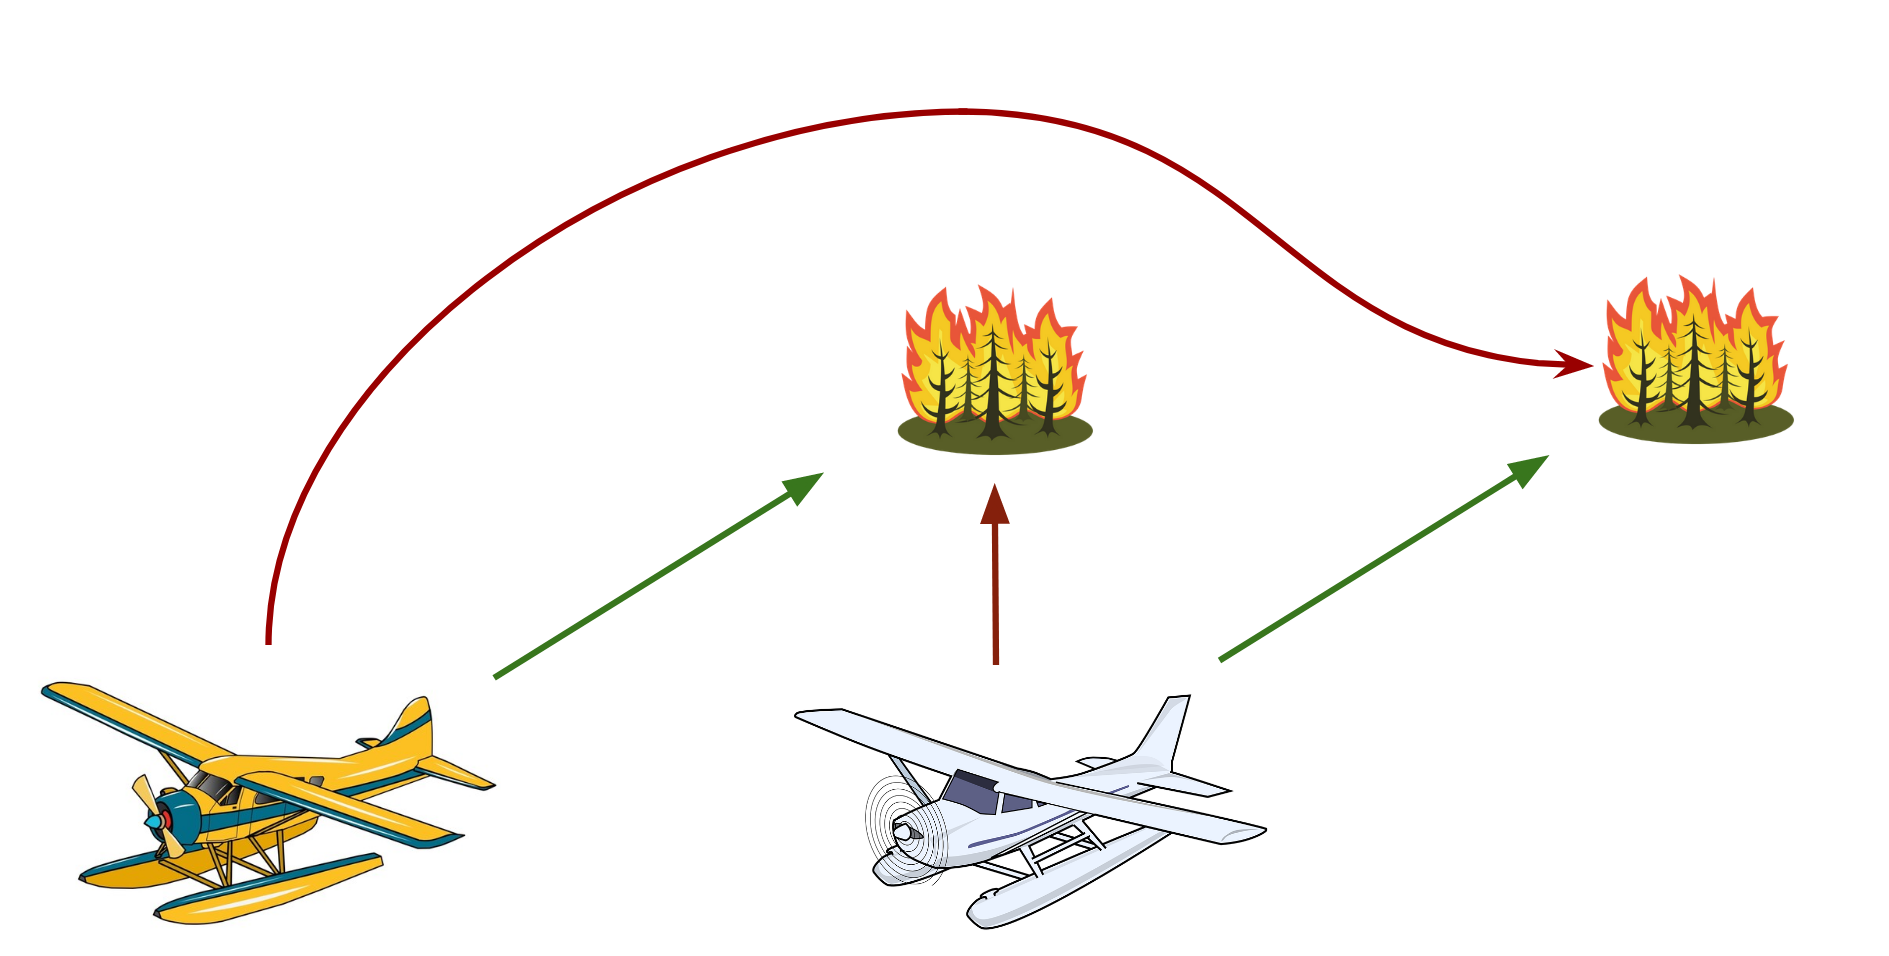
\includegraphics[width=0.74\linewidth]{water_illlu.png}
  \caption{Water-Bomber. Two agents must extinguish all fires; the shared reward
  is granted only when every fire is covered, so the optimal joint behaviour
  (green) often requires one agent to take a longer route to free the other,
  rather than both rushing the nearest fire (red).}
  \label{fig:water}
  \Description{Two water-bomber agents and two fires on a grid; arrows show a
  coordinated assignment of agents to fires versus a greedy one.}
\end{figure}

\paragraph{Simultaneous-Attack.} A one-step, single-state bandit with $N$ agents
and two actions, \emph{attack} or \emph{abstain}. Attacking together succeeds;
attacking without full participation is ``suicidal''. With $K=\sum_i a_i$
attackers we use the reward
\begin{equation}
\label{eq:sim-reward}
r(\mathbf{a})=
\begin{cases}
1 & \text{if } K=N,\\[2pt]
-\,r_{\mathrm{death}}\,K & \text{if } 0<K<N,\\[2pt]
0 & \text{if } K=0,
\end{cases}
\qquad
r_{\mathrm{death}}=\frac{1}{N\,(2^{\,N-1}-1)} .
\end{equation}
This constant (corrected from the earlier $-1/(1-2^{-(N-1)})$, which had the
wrong sign and scale) makes \emph{abstention-vs-coordination} the whole
difficulty: a uniformly random joint policy gets expected return $0$, while the
all-attack optimum gets $1$ (proof in Appendix~\ref{app:reward}). Coordination is
exponentially rare under random play, so the buffer fills with ``failed''
transitions whose value depends entirely on whether teammates would still attack.

\subsection{Protocol.} We use an IQL agent implemented from scratch (PyTorch,
with TorchRL replay buffers), a dueling network for Water-Bomber, $\epsilon$
annealed from $0.99$ to $0.05$, and results averaged over multiple seeds (100 for
Simultaneous-Attack, 10 for Water-Bomber). For each method we report
\emph{average optimality} (normalised return) against environment steps.

\subsection{Findings.}
\paragraph{The problem is real (motivation).} Growing the replay buffer (with the
batch size scaled accordingly) helps \emph{only up to a point} and then
\emph{hurts}, as old transitions become inconsistent with the others' current
policies (Figure~\ref{fig:buffer}). A small buffer avoids the issue but forfeits
sample efficiency---the dilemma this paper targets.

\paragraph{Selection by compatibility helps; raw ratio correction is unstable.}
On both environments, biasing replay towards transitions compatible with the
others' current policies improves sample efficiency over uniform sampling and
over TD-based prioritisation (PER, LaBER), while \emph{directly} multiplying the
loss by $\rho$ destabilises training---the importance ratio spikes
(Figure~\ref{fig:ratios}), confirming the analysis of Section~\ref{sec:ratio}.
The explicit-ratio selection of \cite{foerster2017stabilising} is the special
case of Algorithm~\ref{alg:select} with $A=-\log\rho$; replacing the ratio by the
calibrated conformal score is what extends the method to masked actions and to
settings where $\rho$ is unavailable. The ratio-free conformal instantiation and
the martingale-triggered buffer refresh (Algorithm~\ref{alg:detect}) are the
contributions under active evaluation; we report the protocol above so the
comparison is reproducible.

\begin{figure}[t]
  \centering
  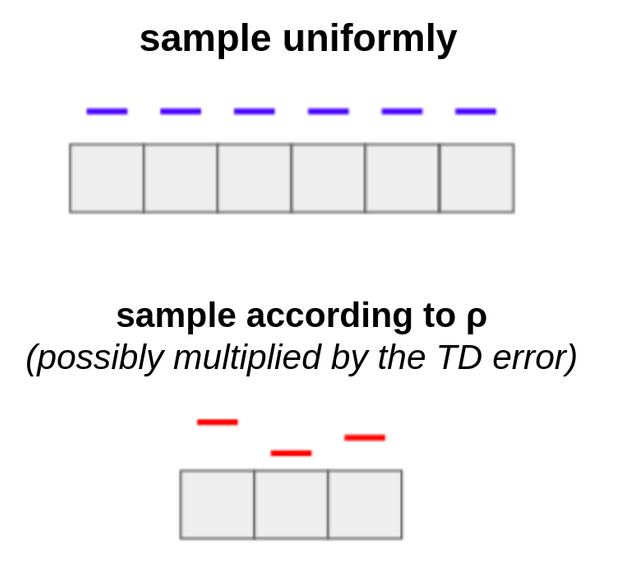
\includegraphics[width=0.74\linewidth]{scheme_final.png}
  \caption{Large-batch-then-subsample replay. A large batch is drawn, each
  transition is scored, and a mini-batch is subsampled towards transitions
  compatible with the others' current policies. The importance ratio $\rho$ is
  one possible score; conformal replay replaces it by a calibrated, ratio-free
  non-conformity score.}
  \label{fig:scheme}
  \Description{Top: a large batch sampled uniformly from the replay buffer.
  Bottom: a smaller batch subsampled according to a per-transition score.}
\end{figure}

\begin{figure}[t]
  \centering
  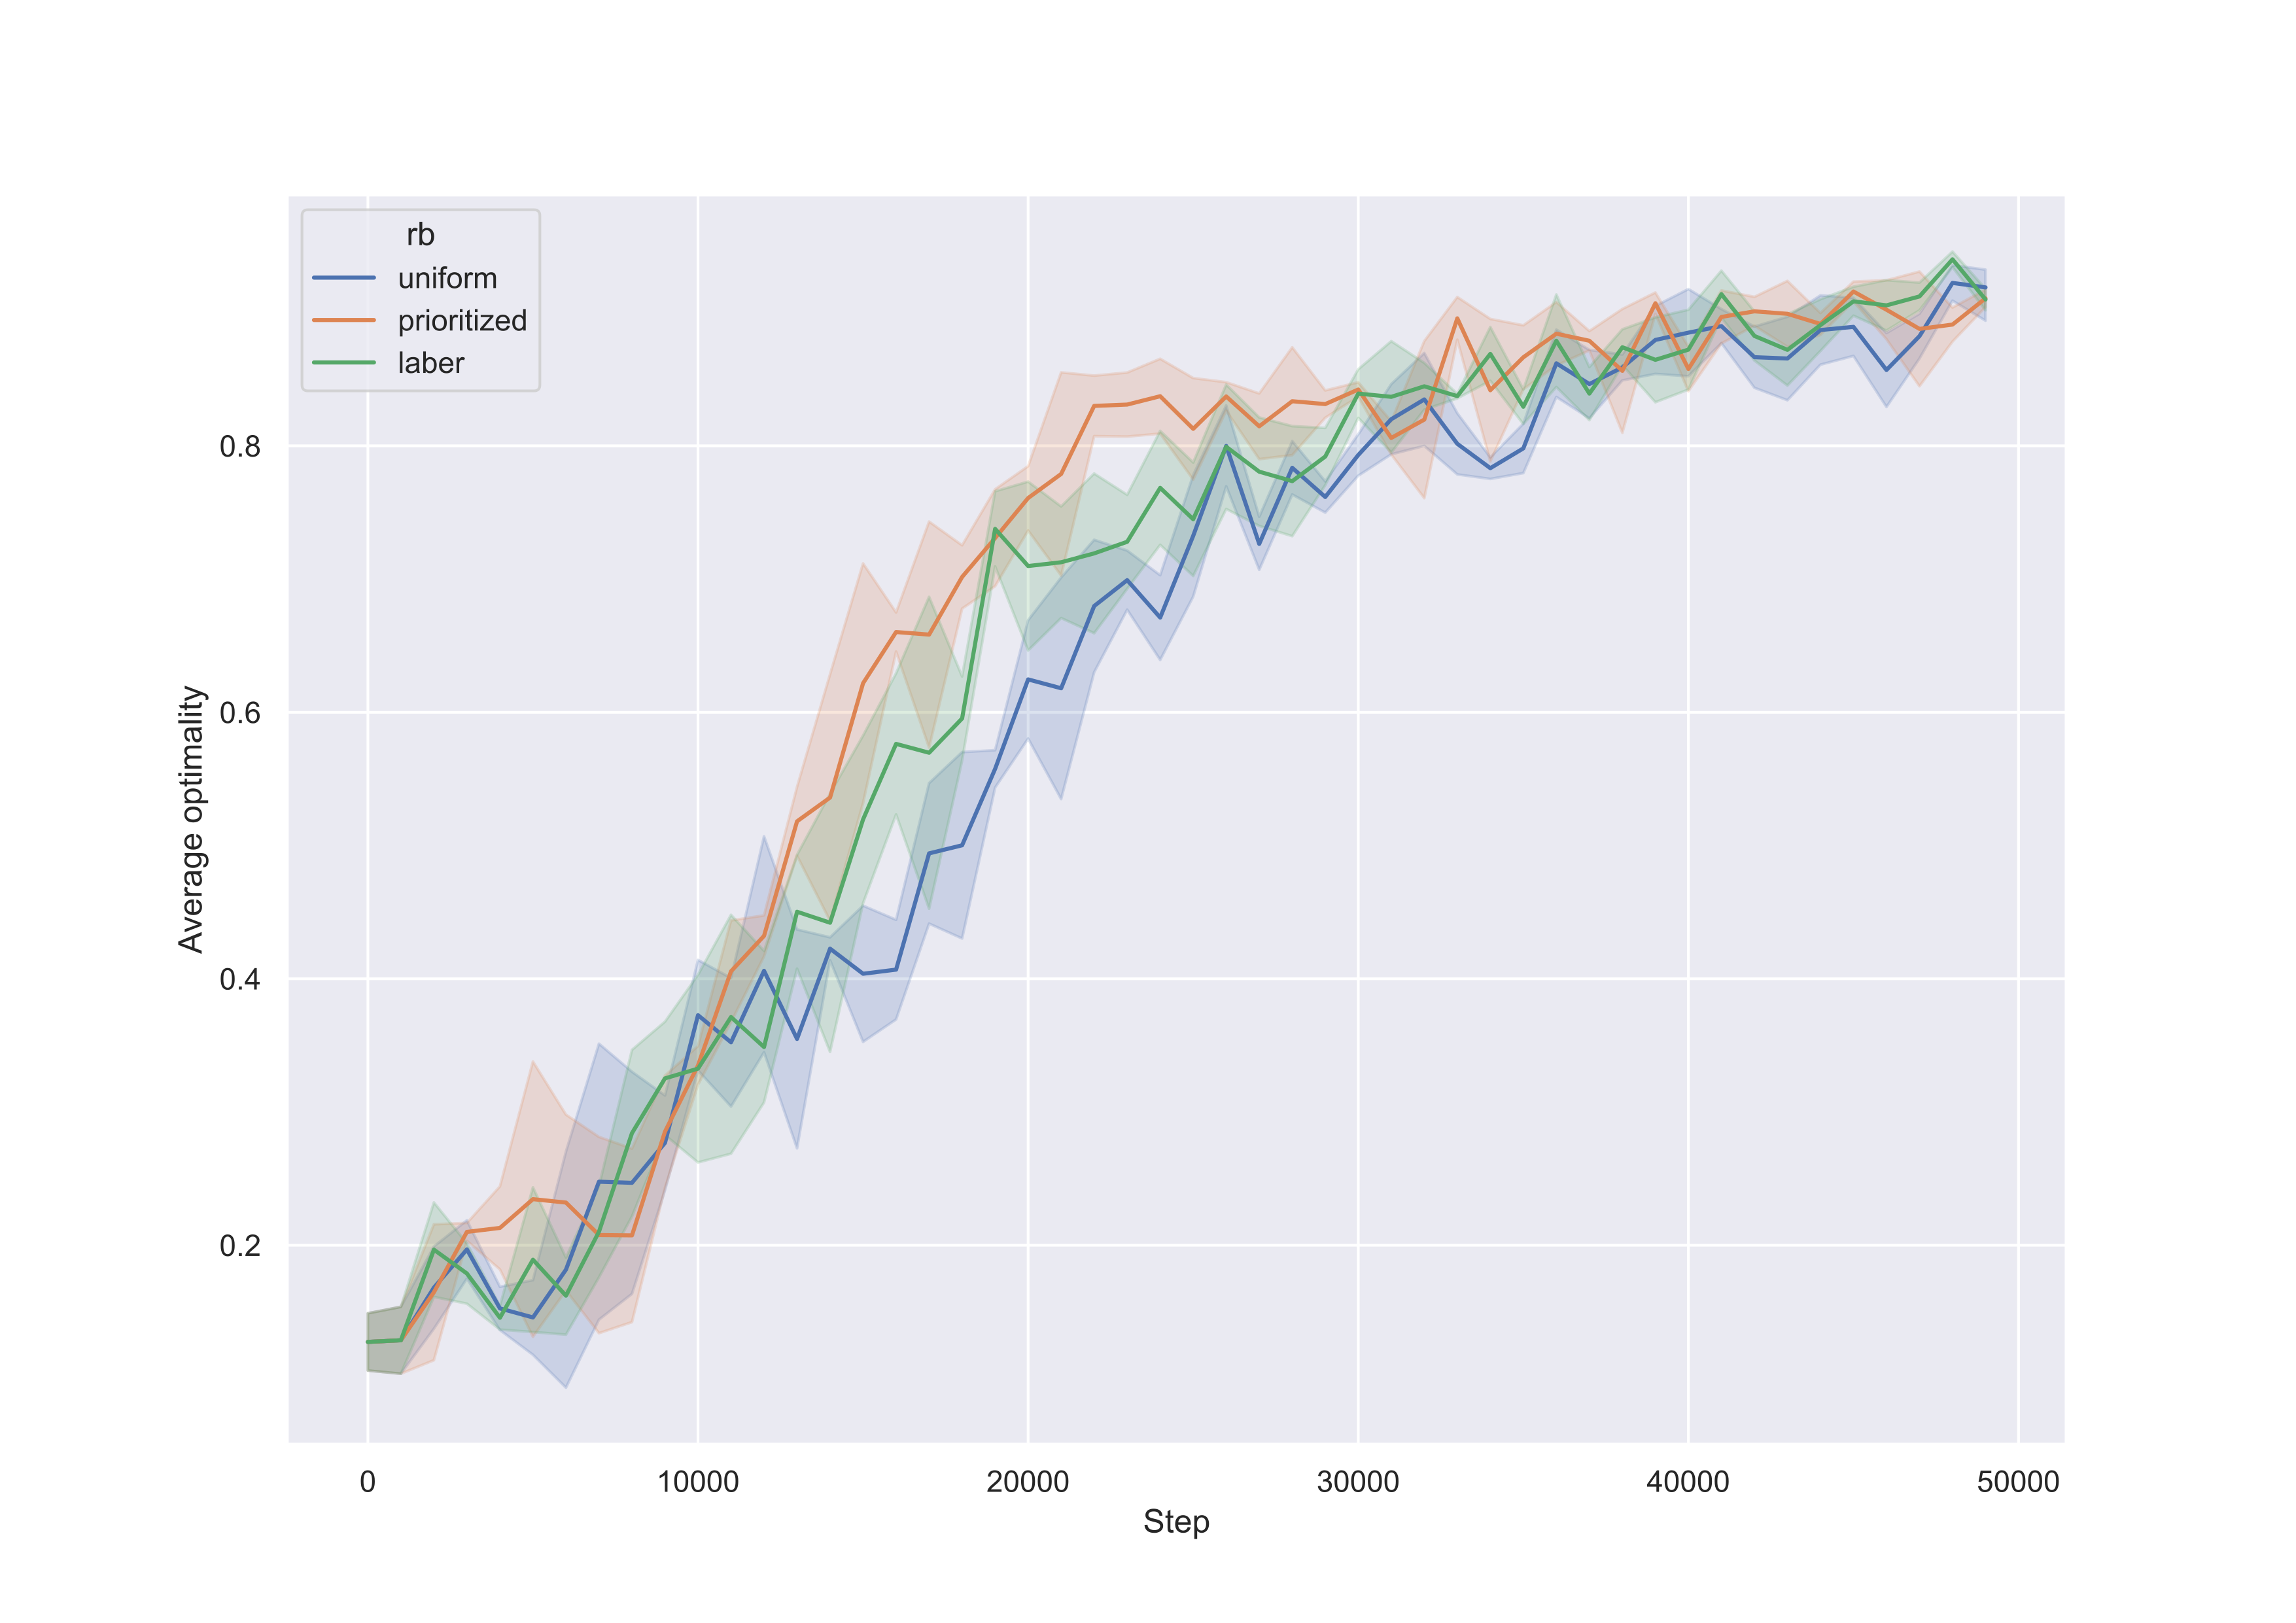
\includegraphics[width=0.92\linewidth]{buffer-water.png}
  \caption{Motivation (Water-Bomber): increasing the replay-buffer size first
  improves then degrades performance, as stale transitions accumulate. The shaded
  band is the inter-seed spread.}
  \label{fig:buffer}
  \Description{Average optimality versus training steps for several buffer sizes;
  the largest buffer eventually underperforms an intermediate one.}
\end{figure}

\begin{figure}[t]
  \centering
  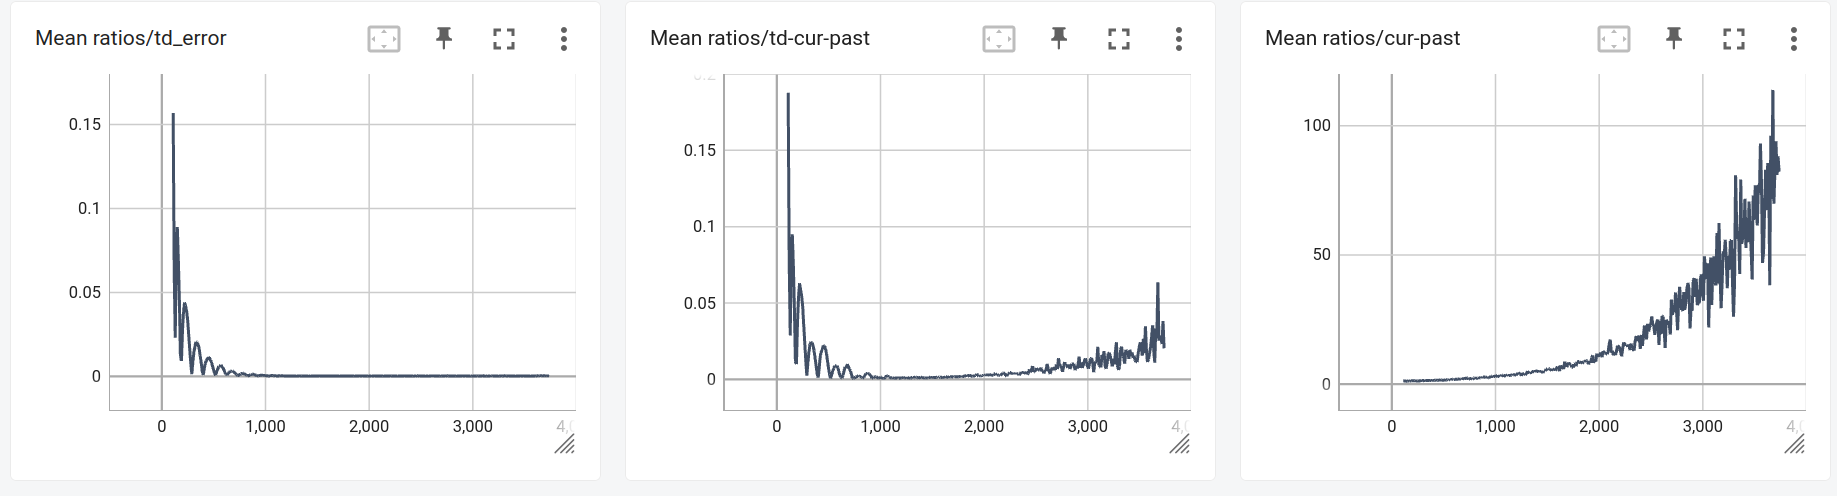
\includegraphics[width=0.86\linewidth]{ratios.png}
  \caption{The importance ratio $\rho$ is heavy-tailed and occasionally huge,
  which makes direct loss correction explode. Conformal calibration uses only the
  \emph{rank} of the score and is immune to this.}
  \label{fig:ratios}
  \Description{Time series of the importance ratio showing rare but very large
  spikes.}
\end{figure}

%%%%%%%%%%%%%%%%%%%%%%%%%%%%%%%%%%%%%%%%%%%%%%%%%%%%%%%%%%%%%%%%%%%%%%%%
\section{Related Work}
The non-stationarity of the perceived environment is a long-standing theme in
cooperative MARL~\cite{matignon2012independent}. \citet{foerster2017stabilising}
stabilise experience replay by conditioning on a low-dimensional fingerprint of
training time and by importance-weighting the loss; we revisit their ratio,
correct its formulation, and remove its dependence on queryable discrete
policies. Value-decomposition methods such as
VDN~\cite{sunehag2018value} and QMIX~\cite{rashid2018qmix}, and the actor-critic
MADDPG~\cite{lowe2017multi}, address credit assignment but still inherit
non-stationary individual learners; PPO-based on-policy
methods~\cite{yu2022surprising} sidestep replay at a sample-efficiency cost.
On the replay side, prioritised experience
replay~\cite{schaul2016prioritized} and LaBER~\cite{lahire2022large} reshape the
sampling distribution by TD error or gradient norm; we borrow their
large-batch machinery but prioritise by \emph{policy conformity} rather than by
error magnitude. Our detection component builds on conformal
prediction~\cite{vovk2005algorithmic,angelopoulos2023gentle} and on conformal
test martingales for change
detection~\cite{vovk2003testing,volkhonskiy2017inductive}, whose anytime validity
follows from Ville's inequality~\cite{ville1939etude,ramdas2023gametheoretic}.

%%%%%%%%%%%%%%%%%%%%%%%%%%%%%%%%%%%%%%%%%%%%%%%%%%%%%%%%%%%%%%%%%%%%%%%%
\section{Conclusion and Future Work}
\label{sec:conclusion}
We recast the reuse of past experience in off-policy MARL as a question of
\emph{conformity to the present} and answered it with conformal prediction. A
single non-conformity score, calibrated into distribution-free $p$-values, both
selects replay transitions that match the other agents' current policies and,
through a conformal test martingale, detects when the perceived environment has
drifted---with an anytime false-alarm guarantee. The construction generalises
importance-ratio reweighting to the realistic cases (masking, partial
observability, continuous actions, black-box teammates) where the ratio is
unavailable or unstable, and we were careful to state what it does and does not
correct.

\balance

Several directions remain. The state-visitation mismatch is untouched and could
be addressed with state-conditional (Mondrian) calibration or with corrections
on $d(s)$. Validity in the dependent RL stream deserves a dedicated analysis,
possibly via e-processes~\cite{ramdas2023gametheoretic}. Finally, the partially
observable setting---where policies condition on histories and the model-based
score~\eqref{eq:score-model} is most useful---is the natural next benchmark,
together with value-decomposition backbones (VDN, QMIX) on SMAC.

\begin{acks}
Anonymised for review.
\end{acks}

%%%%%%%%%%%%%%%%%%%%%%%%%%%%%%%%%%%%%%%%%%%%%%%%%%%%%%%%%%%%%%%%%%%%%%%%
\bibliographystyle{ACM-Reference-Format}
\bibliography{sample}

%%%%%%%%%%%%%%%%%%%%%%%%%%%%%%%%%%%%%%%%%%%%%%%%%%%%%%%%%%%%%%%%%%%%%%%%
\appendix

\section{Convergence of $Q$-learning, corrected}
\label{app:contraction}
The optimal Bellman operator \eqref{eq:bellman} maps an \emph{arbitrary} $Q$ to a
new function (it uses $Q$ on the right-hand side, not $Q^*$). It is a
$\gamma$-contraction in $\lVert\cdot\rVert_\infty$:
\begin{align*}
\big|(\Bop^*Q_1)(s,a)-(\Bop^*Q_2)(s,a)\big|
&=\gamma\Big|\mathbb{E}_{s'}\big[\textstyle\max_{a'}Q_1(s',a')-\max_{a'}Q_2(s',a')\big]\Big|\\
&\le\gamma\,\mathbb{E}_{s'}\big[\textstyle\max_{a'}|Q_1(s',a')-Q_2(s',a')|\big]\\
&\le\gamma\,\lVert Q_1-Q_2\rVert_\infty,
\end{align*}
using $|\max_x f(x)-\max_x g(x)|\le\max_x|f(x)-g(x)|$. Hence
$\lVert\Bop^*Q_1-\Bop^*Q_2\rVert_\infty\le\gamma\lVert Q_1-Q_2\rVert_\infty$ with
$\gamma<1$; the factor $\gamma$ is what makes it a contraction (a
\emph{non-expansion} would not suffice for Banach's theorem). The fixed point is
$Q^*$.

\section{The perceived best-response operator}
\label{app:br}
For fixed $\pi_{-a}$, the operator $\Bop^{\mathrm{BR}}_{\pi_{-a}}$ of
\eqref{eq:br} is a $\gamma$-contraction: the others' actions are averaged out
into the perceived kernel $P^{\pi_{-a}}$ and reward $\bar r^{\pi_{-a}}$, reducing
\eqref{eq:br} to an ordinary optimal Bellman operator on $\mathcal{M}_a(\pi_{-a})$,
to which Appendix~\ref{app:contraction} applies verbatim. Its fixed point
$\Qbr(\cdot;\pi_{-a})$ is the best response of $a$ to $\pi_{-a}$. The MARL Bellman
optimality equation
\[
\Qbr(s,u_a;\picur)=
\mathbb{E}_{\uma\sim\picur}\Big[r_a(s,\mathbf{u})+\gamma\sum_{s'}\mathcal{T}(s'\mid s,\mathbf{u})\max_{u_a'}\Qbr(s',u_a';\picur)\Big]
\]
must be read as a best-response value \emph{conditional on the current others'
policies}, under the quasi-stationary approximation that they are held fixed
during the update---not as a joint-optimal or equilibrium value.

\section{Simultaneous-Attack reward, corrected}
\label{app:reward}
Let each agent attack independently with probability $\tfrac12$ (uniform random
policy), so $K=\sum_i a_i\sim\mathrm{Binomial}(N,\tfrac12)$. With the reward
\eqref{eq:sim-reward},
\[
\mathbb{E}_{U}[r]=\underbrace{1\cdot\mathbb{P}(K=N)}_{=\,2^{-N}}
-\,r_{\mathrm{death}}\sum_{k=1}^{N-1}k\,\mathbb{P}(K=k).
\]
Since $\sum_{k=0}^{N}k\,\mathbb{P}(K=k)=\mathbb{E}[K]=N/2$ and the $k=N$ term is
$N\cdot2^{-N}$,
\[
\sum_{k=1}^{N-1}k\,\mathbb{P}(K=k)=\frac N2-\frac{N}{2^{N}}
=\frac N2\Big(1-2^{-(N-1)}\Big)=\frac{N\,(2^{N-1}-1)}{2^{N}} .
\]
Therefore $\mathbb{E}_U[r]=2^{-N}-r_{\mathrm{death}}\cdot N(2^{N-1}-1)\,2^{-N}$,
which vanishes exactly for
\[
r_{\mathrm{death}}=\frac{1}{N\,(2^{N-1}-1)}>0,
\]
giving a genuine \emph{penalty} ($-r_{\mathrm{death}}K<0$) for partial attacks,
$\mathbb{E}_U[r]=0$ for random play, and $r=1$ for the all-attack optimum. (For
$N=2$: $r_{\mathrm{death}}=\tfrac12$, and
$\mathbb{E}_U[r]=\tfrac14-\tfrac12\cdot\tfrac12=0$.)

\section{Conformal martingale validity}
\label{app:martingale}
Let $\mathcal{F}_t=\sigma(p_1,\dots,p_t)$. If, under $H_0$, each $p_t$ is
conditionally super-uniform, $\mathbb{P}(p_t\le u\mid\mathcal{F}_{t-1})\le u$ for
all $u\in[0,1]$, then for $\varepsilon\in(0,1)$,
\[
\mathbb{E}\big[\varepsilon p_t^{\varepsilon-1}\mid\mathcal{F}_{t-1}\big]
\le\int_0^1\varepsilon u^{\varepsilon-1}\,\mathrm{d}u=1,
\]
so $M_t^{\varepsilon}=\prod_{j\le t}\varepsilon p_j^{\varepsilon-1}$ is a
non-negative supermartingale with $M_0=1$ (a martingale when the $p_t$ are exactly
uniform). Mixing over $\varepsilon$ preserves this. Ville's
inequality~\cite{ville1939etude} for non-negative supermartingales gives
$\mathbb{P}_{H_0}(\sup_{t}M_t\ge1/\delta)\le\mathbb{E}[M_0]\,\delta=\delta$,
which is \eqref{eq:ville} and justifies the anytime threshold $M_t\ge1/\delta$.

\end{document}
%%%%%%%%%%%%%%%%%%%%%%%%%%%%%%%%%%%%%%%%%%%%%%%%%%%%%%%%%%%%%%%%%%%%%%%%
